\section{Results I: Does the Sampler Target the Canonical Law?}
\label{sec:results}
We go from exact to statistical: a local identity (E1), exact stationary laws on small tori (E2), and equilibrium averages at production sizes (E3, E4).

\subsection{Local check of the exchange energy}
\label{sec:results-local}
We enumerated all $\EoneConfigs$ unlike-pair configurations in E1 ($\EoneAdj$ adjacent and $\EoneNonadj$ non-adjacent, over $\EoneDisp$ displacement vectors), and the exact formula \eqref{eq:delta} agrees with the energy difference computed from total energies in every case ($\EoneMismatch$ mismatches). The pair-sum \eqref{eq:pair} agrees with it in every non-adjacent configuration and is off by exactly $-4J$ in every adjacent configuration. The observed set of exact values is $\{-12,\dots,12\}J$ in steps of $4J$ for adjacent pairs and $\{-16,\dots,16\}J$ in steps of $4J$ otherwise, as predicted by \cref{cor:values} (raw data in \texttt{results/paper/E1\_exact\_local.json}). This is an exhaustive computational verification of \cref{prop:delta} on the $6\times6$ torus. The general statement for every $N$ rests on the algebraic proof; the enumeration is an independent check on it.

\subsection{Exact stationary laws on small tori}
\label{sec:results-exact}
\Cref{tab:exact} and \cref{fig:exact} report E2. For the corrected kernel, the exact stationary law coincides with the canonical law to within solver accuracy: the largest total-variation distance over all cases (all sizes, temperatures and both proposal types) is $\EtwoMaxTVcorrect$, and the canonical law is stationary to a residual of at most $\EtwoMaxStatRes$. This is a numerical confirmation of \cref{thm:correct}.

Without the adjacency term the stationary law is far from canonical. With random-pair proposals the total-variation distance ranges from $\EtwoPairMin$ to $\EtwoPairMax$ over the tori and temperatures studied, and with nearest-neighbour proposals from $\EtwoNNMin$ to $\EtwoNNMax$. The mean energy is shifted upwards in every case, because the shortcut over-accepts unfavourable adjacent exchanges. So the loss of reversibility in \cref{prop:flux} does translate into a wrong stationary law; it is not a technicality. These tori are small, with $4/N^2\ge0.25$ of proposals adjacent, so they show the size of the effect when the footprint is of order one, which is what nearest-neighbour proposals give at any $N$. They do not say what happens at production sizes.

\begin{table}[t]
\centering\small
\caption{Exact stationary laws on small tori at $T=2.269$ (E2). $d_{\TV}$ is the total-variation distance to the Boltzmann law $\pi_{\beta,M}$; $\Delta\langle E\rangle$ is the stationary mean energy minus its Boltzmann value ($J=1$). ``Pair'' is the production random-pair proposal, ``NN'' a nearest-neighbour proposal. All temperatures are in \cref{tab:exact-full}.}
\label{tab:exact}
\begin{tabular}{@{}cccc c cc cc@{}}
\toprule
 &  &  &  & correct & \multicolumn{2}{c}{no adj.\ term, pair} & \multicolumn{2}{c}{no adj.\ term, NN}\\
\cmidrule(lr){5-5}\cmidrule(lr){6-7}\cmidrule(lr){8-9}
torus & $M$ & $|\Omega|$ & $T$ & $d_{\TV}$ & $d_{\TV}$ & $\Delta\langle E\rangle$ & $d_{\TV}$ & $\Delta\langle E\rangle$\\
\midrule
$3\times3$ & 3 & 84 & 2.269 & $1\times10^{-14}$ & 0.177 & +1.266 & 0.290 & +1.933 \\
$3\times3$ & 4 & 126 & 2.269 & $4\times10^{-15}$ & 0.227 & +1.324 & 0.359 & +2.259 \\
$4\times4$ & 4 & 1\,820 & 2.269 & $7\times10^{-14}$ & 0.180 & +1.338 & 0.471 & +3.999 \\
$4\times4$ & 6 & 8\,008 & 2.269 & $9\times10^{-14}$ & 0.206 & +1.812 & 0.507 & +5.503\\
\bottomrule
\end{tabular}
\end{table}

\begin{figure}[t]
\centering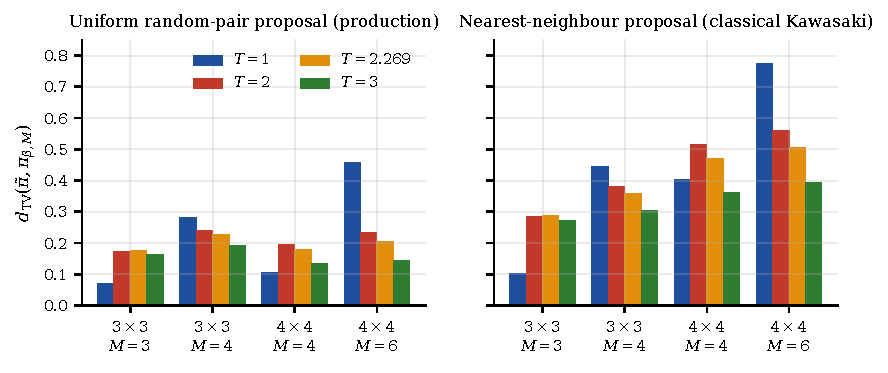
\includegraphics[width=\linewidth]{figures/fig_exact_tv.pdf}
\caption{\textbf{Total-variation distance of the stationary law of the kernel without the adjacency term to the canonical law} on small tori (exact; E2). The corrected kernel has $d_{\TV}<\EtwoMaxTVcorrect$ in all cases (not shown). Left: production random-pair proposal; right: nearest-neighbour proposal.}
\label{fig:exact}
\end{figure}

\subsection{How far does a local error travel?}
\label{sec:results-impact}
At production sizes the question is how much of the one-step perturbation survives in equilibrium averages.

\paragraph{Footprint.} The empirical fraction of adjacent proposals matches $4/N^2$ (\cref{tab:adj}, appendix); at $N=100$ it is $\EthreeAdjHundred$ against $0.0004$, and the fraction of \emph{effective} (unlike-spin) proposals that are adjacent is at most $\EthreeAdjDiffMaxHundred$. The experiment kernels coincide draw-for-draw with the package kernel (equivalence: \EthreeEquivOK).

\paragraph{Equilibrium averages.} \Cref{fig:impact,tab:impact-fit,tab:impact} report E4 (the full table is in the appendix). At $N=8$ and $N=16$ the missing term shifts the mean energy per site upwards by $5.5$--$6.3\%$ and $1.0$--$2.2\%$ respectively (all six comparisons have $|z|\ge5.5$). The ratio of the two effects at $T=1.5$ is $\EfourSmallRatio$, close to the factor $4$ expected if the effect scales with the footprint $N^{-2}$. At $N\ge32$ we cannot distinguish the shift from zero: $\EfourCountLargeSig$ of $\EfourCountLarge$ comparisons has $|z|>1.96$, about what nine comparisons produce under the null. A weighted fit $\Delta\langle e\rangle=c/N^2$ over all five sizes (\cref{tab:impact-fit}) gives $c=4.4\pm0.2$, $3.7\pm0.1$ and $2.35\pm0.10$ at $T=1.5$, $\Tc$ and $3$, with fit $p$-values $0.22$, $0.02$ and $0.44$. The $N^{-2}$ law describes the data at two temperatures and is in moderate tension with them at $T=\Tc$. Extrapolating, the predicted shift at $N=32$ is about $\EfourPredThirtyTwo$ against a standard error of $\EfourSeThirtyTwo$ per comparison, below our resolution.

What this establishes is limited. The kernel without the adjacency term is wrong, its effect is measurable and large at small $N$, and it scales as the footprint suggests. We do not claim it changes macroscopic results at $N\ge32$ under random-pair proposals; our replication has too little power to say. We did not analyse its effect on variances or higher moments, which are what the variance-peak estimator uses.

\begin{figure}[t]
\centering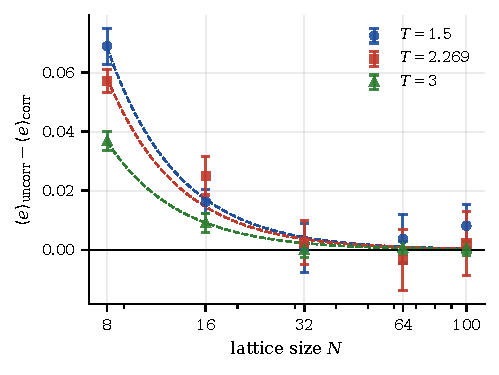
\includegraphics[width=0.62\linewidth]{figures/fig_adjacency_impact.pdf}
\caption{\textbf{Effect of omitting the adjacency term on the mean energy per site} ($f=1/2$; E4). Points: difference of replicate means with $95\%$ intervals ($1.96$ Welch standard errors); dashed: weighted fit $c/N^2$. Vertical axis is symmetric-log.}
\label{fig:impact}
\end{figure}


\begin{table}[t]
\centering\small
\caption{E4: weighted fits $\Delta\langle e\rangle=c/N^2$ over $N\in\{8,16,32,64,100\}$. $\chi^2$ (degrees of freedom) and $p$-value of the fit; $\chi^2_0$ and $p_0$ for the null $c=0$ (5 d.o.f.).}
\label{tab:impact-fit}
\begin{tabular}{@{}cccccrc@{}}
\toprule
$T$ & $c$ & s.e. & $\chi^2$ (d.o.f.) & $p$ & $\chi^2_0$ & $p_0$\\
\midrule
1.5 & 4.38 & 0.19 & 5.7 (4) & 0.22 & 565 & $<10^{-6}$ \\
2.269 & 3.73 & 0.13 & 11.2 (4) & 0.02 & 880 & $<10^{-6}$ \\
3 & 2.35 & 0.10 & 3.7 (4) & 0.44 & 521 & $<10^{-6}$\\
\bottomrule
\end{tabular}
\end{table}
